\documentclass{standalone}
\usepackage{circuitikz}
\usepackage{amsmath, amssymb}
\usepackage{siunitx}
\begin{document}
	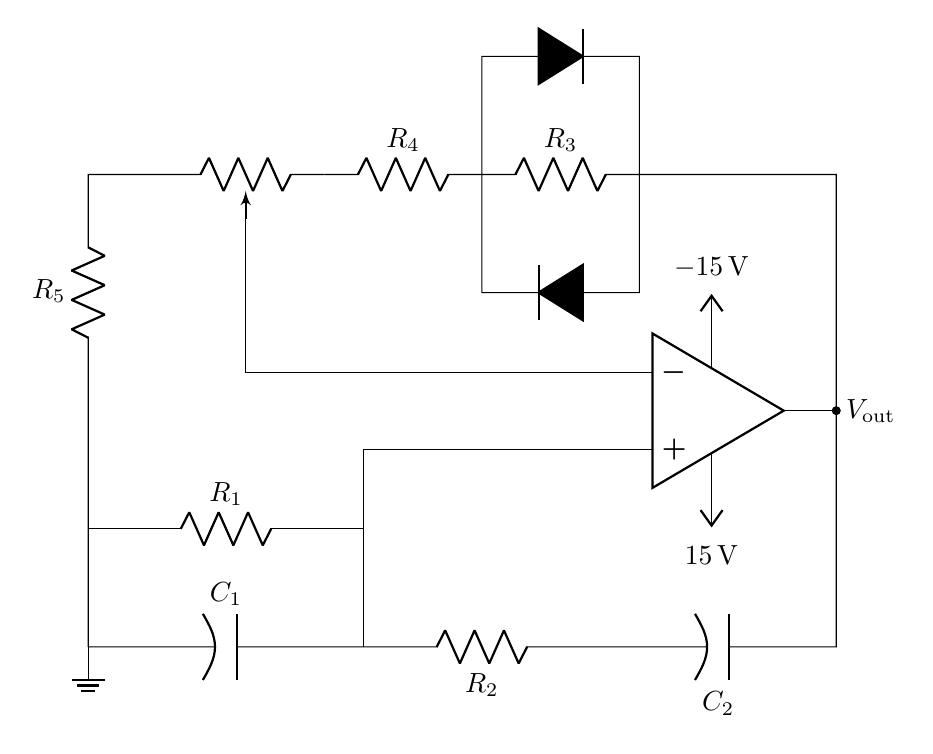
\begin{tikzpicture}
		\draw (0,0) node [op amp] (op) {};
		\draw (op.up) -- ++(0,0.5) node[vcc]{\SI{-15}{\volt}};
		\draw (op.down) -- ++(0,-0.5) node[vee]{\SI{15}{\volt}};
		\draw (op.out) -- (1.5,0);
%		\draw (-9, 3) node[ground] {} to[R, l=$ R_{3} $] ++(2,0) to[pR] ++(2,0)
		\draw (-5,3) to[pR] ++(-2,0) -- ++(-1,0) to[R, a=$ R_{5} $] ++(0,-3) --
		++(0,-3) node[ground] {};
		\draw (-5,3)
		to[R, l=$ R_{4} $] ++(2,0) to[R, l=$ R_{3} $] ++(2,0) -- ++(0, -1.5) to[D*]
		++(-2,0) -- ++(0, 3) to[D*] ++(2,0) -- ++(0,-1.5) -| (1.5,0);
		\draw (op.-) -| (-6, 2.7);
		\draw (1.5, 0) -- ++(0,-3) to[pC, l=$ C_{2} $, invert] ++(-3,0)
		to[R, l=$ R_{2} $] ++(-3,0);
		\draw (-4.5, -3) to[pC, a=$ C_{1} $, invert] ++(-3.5,0);
%		\draw (-4.5, -3) -- ++(0,-1.5) to[R, a=$ R_{1} $] ++(-3,0) -- ++(0,1.5) -- ++(-1, 0) node[ground] {};
		\draw (op.+) -| (-4.5, -3);
		\draw (-4.5, -1.5) to[R, a=$ R_{1} $] ++(-3.5,0);
		
		\filldraw (1.5, 0)  circle [radius=0.05] node[right] {$ V_{\rm out} $};
	\end{tikzpicture}
\end{document}